\section{Enhanced techniques}\label{sec:enhanced}
\subsection{Combining different data types - MT 1d inversion}\label{sec:mt1d}
File \file{doc/tutorial/code/enhanced/mt1dinv0.cpp}\\
In magnetotelluric (MT) inversion for every period an amplitude $\rho^a$ and a phase $\phi$ is computed from the electric and magnetic registrations. The file \file{1000\_100\_1000\_n5\_1.dat} contains a synthetic three layer case of 1000$\Omega$m-100$\Omega$m-1000$\Omega$m with 5\,\% Gaussian noise on the $\rho^a$ and 1 degree on the phases.
The three columns $T$, $\rho^a$ and $\phi$ are read extracted as vectors by
\begin{lstlisting}
    RMatrix TRP; //! real matrix with period(T), resistivity(R) & phase(P)
    loadMatrixCol( TRP, dataFileName ); //! read column-based file
    size_t nP = TRP.rows(); //! number of data
    RVector T( TRP[0] ), rhoa( TRP[1] ), phi( TRP[2] ); //! columns
\end{lstlisting}
It is based on the forward operator \lstinline|MT1dModelling| in \file{src/em1dmodelling.h/cpp}, giving back a vector that consists of the amplitudes and phases for each period. 
Of course both have completely different valid ranges. 
The phases a linearly related between 0 and $\pi/2$, whereas the amplitudes are usually treated logarithmically.
On the (1d block) model side, thickness and apparent resistivity use log or logLU transforms as done for DC resistivity.
\begin{lstlisting}
    /*! Model transformations: log for resistivity and thickness */
    RTransLog transThk;
    RTransLogLU transRho( lbound, ubound );
    /*! Data transformations: log apparent resistivity, linear phases */
    RTransLog transRhoa;
    RTrans transPhi;
\end{lstlisting}
Since amplitudes and phases are combined in one vector, we create a cumulative transformation of the two by specifying their lengths. 
Similarly, the assumed relative error of the $\rho^a$ and $\phi$ are combined using a cat command.
\begin{lstlisting}
    CumulativeTrans< RVector > transData; //! combination of two trans
    transData.push_back( transRhoa, nP ); //! append rhoa trans (length nP)
    transData.push_back( transPhi, nP );  //! append phi trans
    RVector error( cat( RVector(nP,errRhoa/100), RVector(errPhase/phi) ) );
\end{lstlisting}

Similar to DC resistivity inversion, we create a 1d block mesh, initialise the forward operator and set up options for the two regions (0-thicknesses,1-resistivities).
Starting values for the $\rho_i$ and $d_i$ are computed by the mean apparent resistivity and an associated skin depth.
\begin{lstlisting}
    MT1dModelling f( T, nlay, false );
    double medrhoa = median( rhoa ); //! median apparent resistivity
    double medskindepth = sqrt( median( T ) * medrhoa ) * 503.0; //!skin d.
    f.region( 0 )->setTransModel( transThk ); //! transform
    f.region( 1 )->setTransModel( transRho );
    f.region( 0 )->setConstraintType( 0 ); //! min. length
    f.region( 1 )->setConstraintType( 0 );
    f.region( 0 )->setStartValue( medskindepth / nlay );
    f.region( 1 )->setStartValue( medrhoa );
    /*! Real valued inversion with combined rhoa/phi and forward op. */
    RInversion inv( cat( rhoa, phi ), f, verbose, dosave );
\end{lstlisting}

The rest is done as for DC resistivity block inversion.
In Figure~\ref{fig:mt1dblock-resres} the inversion result and its resolution matrix is shown.
The model is very close to the synthetic one and represents an equivalent solution.
This is also represented by the resolution matrix, where $\rho_1$, $\rho_3$ and $d_1$ are resolved almost perfectly, whereas $\rho_2$ and $d_2$ show slight deviations.
\begin{figure}[htbp]
\centering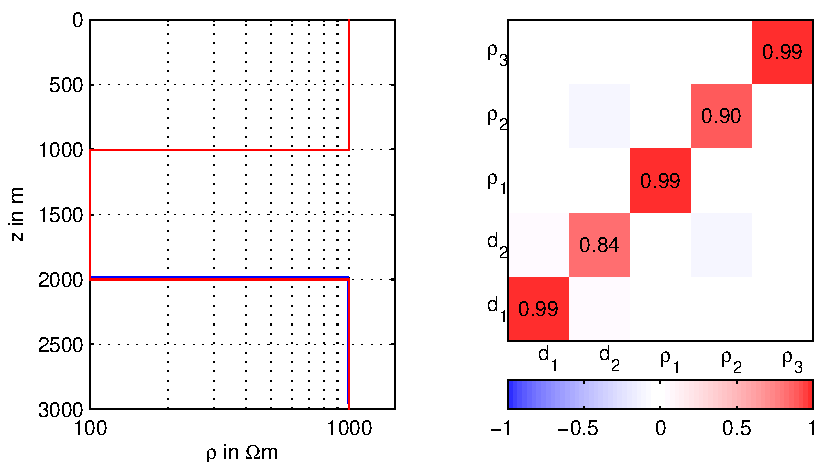
\includegraphics[width=0.7\textwidth]{mt1dblock-resres}\\[-3ex]
~\hfill a\hfill ~ \hfill ~~~~~b \hfill ~ \hfill ~ \hfill ~
\caption{a) Block 1d resistivity inversion result (red-synthetic model, blue-estimated model)) and b) resolution matrix}\label{fig:mt1dblock-resres}
\end{figure}

One can easily test the inversion only based on $\rho^a$ or $\phi$ by increasing the errors of the others by a large factor.
According to (\ref{eq:phid}) the corresponding weight goes to zero.
By skipping $\phi$ the model deviates slightly and the cell resolutions for $\rho_2$ and $d_2$ decrease to 0.9 and 0.86, respectively. If the $\rho^a$ are neglected the solution becomes obviously non-unique. Only $d_1$ is determined pretty well, the other parameters obtain cell resolutions of 0.6-0.8. Note also that for local regularisation the resolution does not contain the resolution of the preceding models \citep{friedel03}.

%%%%%%%%%%%%%%%%%%%%%%%%%%%%%%%%%%%%%%%%%%%%%%%%%%%%%%%%%%%%%%%%%%
\subsection{Combining different parameter types - offsets in travel time}\label{sec:ttoffset}
Next, we consider a 2d travel-time tomographic problem.
In the library there is a forward operator called \cw{TTDijkstraModelling}, which is using a Dijkstra \citep{dijkstra} algorithm that restricts the ray paths to mesh edges. Although this is only an approximation, it is sufficiently accurate for high-quality meshes.
Assume the zero point (shot) of the traces is not exactly known. This might be due to long trigger cables, problems in the device or placing besides the profile.
Aim is to include an unknown delay for each shot position into the inversion\footnote{A similar problem is the issue of static shift in MT inversion caused by local conductivity inhomogeneity, which shifts the apparent resistivity curves.}.

First, we derive a new forward modelling class \cw{TTOffsetModelling}  from the existing \cw{TTDijkstraModelling} (abbreviated by \cw{TTMod}) since we want to use their functionality.
Additionally to the existing class we need the number of shot positions and a zeroth order mesh holding the offset values for them added to the original mesh.
\begin{lstlisting}
class TTOffsetModelling : public TTMod {
public:
    TTOffsetModelling( Mesh & mesh, DataContainer & data )
      : TTMod( mesh, data ) {
        std::vector < size_t > sources( mesh_->findNodesIdxByMarker(-99) );
        int nShots_ = sources.size();
        for ( size_t i = 0; i < dataContainer.electrodeCount(); i ++ ){
            offsetMesh_.createCell( 3 );
        }
        regionManager_->createRegion( 3, offsetMesh_ );			 
    }
    virtual ~TTOffsetModelling(){ }
    RVector response( const RVector & model );
    void createJacobian( H2Matrix & jacobian, const RVector & model );
protected:
    int nShots_;
    Mesh offsetMesh_;
}
\end{lstlisting}

The two functions \cw{response} and \cw{createJacobian} need to be overwritten.
However we want to expand the original functions by the changes needed.
This is straight forward for the response vector.
First part of the model is the slowness vector whose response is calculated calling the original function.

\begin{lstlisting}
    RVector TTOffsetModelling::response( const RVector & model ){
        //! extract slowness from model and call old function
        RVector slowness( model, 0, model.size() - nShots_ );
        RVector resp = TTMod::response( slowness );
        //! extract offsets from model and add to reponse
        RVector offsets( model, model.size() - nShots_, model.size() );
        for( int i = 0; i < DataContainer.size(); i++ ){
           resp[ i ] += offsets[ DataContainer.a( i ) ];
        }
        return resp;
    }
\end{lstlisting}

For the Jacobian the case is a bit more complicated.
Instead of increasing the size of the matrix a-posteriori, we define a new matrix type \cw{H2Matrix} consisting of two horizontally concatenated matrices.
The first is the normal way matrix holding the path lengths.
Second is a matrix with a value of one in the position of the shot number and 0 elsewhere.

\begin{lstlisting}
    RVector TTOffsetModelling::createJacobian( H2Matrix & jacobian, 
                                          const RVector & model ){
        //! extract slowness from model
        RVector slowness( model, 0, model.size() - nShots_ );
        RVector resp = TTMod::createJacobian( jacobian.H1(), slowness );
        //! 
        for( int i = 0; i < nShots_; i++ ){
            //! set specific values to 1
        }
    }
\end{lstlisting}

See appendix on matrices \ref{app:matrix} for existing matrix types.

%%%%%%%%%%%%%%%%%%%%%%%
\subsection{What else?}
\begin{itemize}
	\item Full waveform TDR inversion?
	\item Gravity 2d or 3d inversion?
	\item what is enhanced?
\end{itemize}
